\documentclass{standalone}
\usepackage{tikz}
\tikzset{         block/.style = {draw, fill=white, very thick, rectangle, minimum height=1cm, minimum width=2cm},
}
\begin{document}
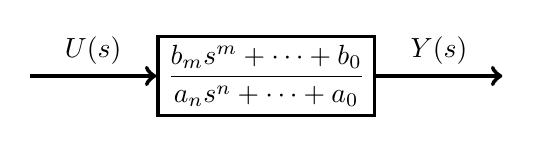
\begin{tikzpicture}[scale=2]
    \node[block](h)at(0,0){$\displaystyle\frac{b_ms^m+\cdots+b_0}{a_ns^n+\cdots+a_0}$};
    \draw[->,ultra thick](-1.5,0)--(h.180)node[midway, above]{$U(s)$};
    \draw[->,ultra thick](h.0)--(1.5,0)node[midway, above]{$Y(s)$};
\end{tikzpicture}
\end{document}